\chapter{Literature Review}
\label{chap:litterature}

\section{Related work}

\subsection{Group Key Management}

\subsubsection{Mathematical approach}

GKM as a problematic has several dimensions and different types of issues to consider and tackle. Some research focused on reliable key generation issues in GKM. In \cite{zhan_novel_2017}, the authors analyzed the impact of key management techniques on connectivity and efficiency in Wireless Sensor Networks (WSNs). In order to address the issue, they propose a key generation method based on system of equations. Considering how the work was carried out to tackle poor connectivity and multiple forwarding issues, the solution is actually pretty scalable. The paper considers a system of u equations with v variables as follows:

\begin{math}
	\Phi^{\left(v\right)} =
	\left\{
	\begin{array}{l}
		\phi_1 \left(x_1, x_2, \ldots, x_v\right) = 0\\
		\vdots \\
		\phi_u \left(x_1, x_2, \ldots, x_v\right) = 0
	\end{array}
	\right.
\end{math}\\

This equation has one unique solution which will be used to generate a shared secret key to be shared among the network’s nodes. Solutions of equation systems actually constitute the associated keys, from which we then generate those secret keys. Two systems of equations were considered: linear equations and polynomial equations. The first system was recommended over the second one, due to its lower complexity.

Another solution based on the Kronecker product was proposed in \cite{tsai_key_2017}. Authors of the paper already proposed CRAPPY (Constrained RAndom Perturbation-based Pairwise keY establishment), a key establishment protocol for WSNs. However the latter doesn’t consider heterogeneity in IoT networks, neither scalability related issues. Considering the exponential growth of IoT devices and their diversity, this protocol is simply impractical. The authors utilize the matrix Kronecker product to generate private and public keys for the network’s nodes. We cite the property:

\begin{quote}
	\begin{math}
		If\; A \in \mathcal{R}^{\sqrt{m} \times \sqrt{m}} \; and\; A \in \mathcal{R}^{\sqrt{n} \times \sqrt{n}} \; are\; symmetric,\; then\; A \otimes G\; is\; symmetric. 
	\end{math}
%If $A \mathcal{R}^{\sqrt{m}\times\sqrt{m}}$ and $A \mathcal{R}^{\sqrt{n}\times\sqrt{n}}$ are symetric, then $A\otimesG$ is symetric. 
\end{quote}

Therefore, we are able to generate couples of keys for each of the network’s nodes. The system assigns a couple of keys, private and public, to each node. The paper more in depth how the system exactly works. Its resilience resides in the difficulty of reconstructing the Kronecker product by any of the sensor nodes. Besides, it factorizes asymmetric encryption for messages exchange, which is rather safer than symmetric encryption.

\subsubsection{Key management architectures}

Tiloca and Dini in \cite{tiloca_grep_2016} proposed GREP, a group rekeying protocol. The protocol assumes the presence of an IDS. The latter’s main function is to detect eventual attacks on the network, in order to identify compromised nodes to be evicted. However, the paper points out that nodes suspected by the IDS as compromised are considered unreliable, and therefore will also be evicted by the Group Membership Service. Thus, each node compromising or suspicion will probably induce the whole rekeying upon leaving process.
Yet this topic is not covered in the paper. Even though it’s beyond the scope the treated problematic, the service role in the overall problem seems under-valued. Actually, the quality of the IDS can significantly influence the global efficiency reference criteria of the rekeying protocol. On one side, a well-designed IDS is able to efficiently detect which nodes exactly are compromised. As suspected nodes are also to be evicted, the IDS can eventually raise some false alarms. Hence, optimising the IDS accuracy will decrease the number of possible false alarms, and so the number of useless rekeying process operations with all the cost that comes with. On the other side, some attack scenarios involve compromising one node at first, before propagating in the network reaching others. If the IDS is efficient enough to provide early detection of compromised nodes, it can lower the rekeying process’ cost which should follow. Regarding the rekeying upon leaving process detailed in the paper, having few compromised nodes belonging to a limited number of subgroups is clearly an advantage.
So we can see here that IDS role can be crucial in the key management protocol, as it can significantly contribute in the saving of the network’s bandwidth and limiting the node’s energy drainage.

The rekeying process, whether upon a joining node or a leaving one, is based on one central element which is the refreshing key $K_R$. The latter is then employed in order to generate almost all new tokens and encryption keys for group, subgroup and pairwise communications. However, the paper doesn’t explain precisely how this $K_R$ is generated, nor the measures taken to secure its generation.

Kung and Hsiao \cite{kung_groupit_2018} proposed GroupIt, a two-tier GKM architecture. It supports multi-group networks, and embeds its own methodologies to handle device membership updates. The upper tier is resposible for key management between different groups. The lower tier is however responsible for key management within groups. The architecture considers two types of groups: device groups and user groups. Device groups incorporate devices based on their technical functionalities and security requirements. The systems also establishes user groups which contain one or multiple device groups. A device group can belong to different user groups, and every user is assigned to one and only one user group.

\begin{figure}[htbp]
	\centerline{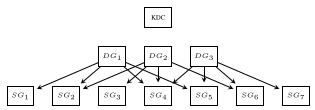
\includegraphics[scale=0.75]{figures/groupit.png}}
	\caption{Source \cite{kung_groupit_2018}: GroupIt initial structure overview}
	\label{groupit}
\end{figure}

Every device group has its own GKM scheme, such as Logical Key Hierarchy (LKH). But above all these groups, we have a KDC which provides keys for inter-group communications. Although the proposed system considers mechanisms to ensure secure communications, forward and backward secrecy, and resistance against collusion attacks, it still has a central problem: the whole lies on the KDC. This centralization generates a single point of failure within the architecture. That’s why we need to dig deeper into decentralization issues and proposed solutions.

\subsubsection{Decentralized key management}
\label{subsec:decentralized}

Several solutions for decentralized Key Management were considered. Veltri et al. \cite{veltri_novel_2013} proposed a batch-based group key management. The solution looked more at distributing the rekeying operations as events. The protocol relies on a central Key Distribution Center though, so the key management as a role remains centralized after all. Dammak et al. \cite{dammak_decentralized_2020} proposed a decentralized Group Key Management architecture. This hierarchical architecture relies on several Key Distribution Centers (SKDCs) with a central Key Distribution Center (KDC) on top. This solution already distributes the task of key management, but only partially. The SKDCs aren’t completely autonomous regarding the KDC and are still dependant on it. Hence, the issue of single point of failure persists. The Blockchain technology was also considered \cite{truong_towards_2019, kouicem_decentralized_2019} to address the problem. The use of Blockchain requires from every node to keep its own copy of the ledger. This solution takes us from a point where a single entity is handling the key management, to a situation where practically all network nodes are acting as Key Manager. Giving the need to add a ledger block on every rekeying operation, this introduces a significant processing overhead (due to required Proof-of-Works) and networking overhead (due to required ledger update).

A cluster based Key Management solution was suggested by Khan and Anandharaj in \cite{feroz_khan_cognitive_2019}. It uses a cognitive key management technique to increase energy efficiency and scalability. The work considers Cluster Head (CH) election process and highlights the need for cluster maintenance. However, the proposed election process adopts a classical network routing approach. Besides, it does not consider security risks related to this cluster based scheme, nor its mitigation. The algorithm’s analysis is focused on energy efficiency, with few regard to security.

\subsection{Cluster Head selection}
\label{subsec:ch}

Actually, Cluster Head based architectures have been long studied. Heinzelman et al. \cite{heinzelman_energy-efcient_2000} considered network clustering as a network routing solution. They proposed LEACH (Low-Energy Adaptive Clustering Hierarchy) to address the energy dissipation issue in node-to-base station communications. It suggests a cluster-divided network with one node in every cluster acting as local Base Station (BS), dubbed CH. Different CHs collect data from their fellow cluster members, and transmit them to the main BS. Extensions of this scheme were then proposed \cite{al-baz_new_2018, kang_distance_2012}. Other algorithms for CH selection seeking to optimise energy consumption and load-balancing were suggested in \cite{behera_residual_2019, jia_dynamic_2016}. These algorithms utilize node’s energy capabilities to balance probabilities for CH selection among other cluster nodes. But all these studies aim to optimise energy performances with no regard to security. They were basically developed to save radio transmission overhead, thereby they deal with network and data routing oriented problems. However, our interest for this scheme is foremost driven by our need to solve the Key Management problem for group communication and provide a decentralized model for it. Moreover, the CH election in previous works is based on energy, communication and networking related criteria. Besides, they mainly consider homogeneous environments in which CH are to communicate with a fixed Base Station (BS) for application reasons. Hence, the described models are not necessarily fit for use as a security oriented scheme (cryptographic key management in our case) for heterogeneous IoT networks. In our use case, we tend more to think over the architecture from a security point of view.

\section{Identification of remaining challenges}

In literature review, we considered both, decentralized key management as a challenge and network clustering as a scheme. Based upon this, we can notice that these works are mostly energy performance oriented. We need key management and cryptographic keys to ensure security in the first place. Despite that the main problematic, key management, is actually a security problematic, relevant researches are usually conducted with a networking and energy mindset, sometimes discarding security concerns \cite{ziegeldorf_privacy_2014, zhang_iot_2014, khan_iot_2018}. This work aims at bringing back the security perspective to the front view, besides the energy aspect. Thus to propose a solution which offers a satisfactory security-efficiency compromise.